\section*{Question 1}
We consider a multivariate version of ridge regression where $X : \Omega \rightarrow \mathbb{R}^{d}$, $Y : \Omega \rightarrow \mathbb{R}^{q}$, $\beta_{0} \in \mathbb{R}^{q}$, and $b$ is a $d \times q$ matrix, with predictor $f : \mathbb{R}^{d} \rightarrow \mathbb{R}^{q}$ given by:
\begin{center}
    $f(x) = \beta_{0} + b^{T}X$
\end{center}
Introducing a $d \times d$ positive semi-definite symmetric matrix $D$, we consider penalized least-square estimators $\hat{\beta}_{0}$ and $\hat{b}$ given by minimizers of:
\begin{center}
    $F(\beta_{0}, b) = \sum\limits_{k=1}^N|y_{k} - \beta_{0} - b^{T}x_{k}|^{2} + \lambda$ trace($b^{T}Db$)
\end{center}
where ($x_{1}, y_{1}$),...,($x_{N}, y_{N}$) are the training data.
\vspace{5mm}

(1.1) Let $\bar{x}$ and $\bar{y}$ denote the average of $x_{1}$,...,$x_{N}$ and $y_{1}$,...,$y_{N}$ respectively, and denote by $\mathcal{Y}_{c}$ and $\mathcal{X}_{c}$ the matrices:
\begin{center}
$\mathcal{Y}_{c} = 
\begin{pmatrix}
(y_{1} - \bar{y})^{T} \\
\vdots \\
(y_{N} - \bar{y})^{T}
\end{pmatrix}
,
\mathcal{X}_{c} = 
\begin{pmatrix}
(x_{1} - \bar{x})^{T} \\
\vdots \\
(x_{N} - \bar{x})^{T}
\end{pmatrix}$
\end{center}
To find $\hat{b}$ and $\hat{\beta}_{0}$ such that $F(\beta_{0}, b)$ is minimized, we take the partial derivative of $F$ with respect to $\beta_{0}$ and set it equal to 0 as such:
\begin{center}
    $0 = -2\sum\limits_{k=1}^N|y_{k} - \hat{\beta}_{0} - \hat{b}^{T}x_{k}|$
\end{center}
We can solve this equation for $\hat{\beta}_{0}$ as follows:
\begin{center}
    $0 = \sum\limits_{k=1}^N y_{k} - N\hat{\beta}_{0} - \sum\limits_{k=1}^N \hat{b}^{T}x_{k}$

    $0 = N\hat{\beta}_{0} - \sum\limits_{k=1}^N (y_{k} - \hat{b}^{T}x_{k})$

    $N\hat{\beta}_{0} = \sum\limits_{k=1}^N (y_{k} - \hat{b}^{T}x_{k})$

    $\hat{\beta}_{0} = \frac{1}{N}\sum\limits_{k=1}^N (y_{k} - \hat{b}^{T}x_{k})$

    $\hat{\beta}_{0} = \frac{1}{N}\sum\limits_{k=1}^N y_{k} - \hat{b}^{T} \frac{1}{N}\sum\limits_{k=1}^N x_{k}$

    $\hat{\beta}_{0} = \bar{y} - \hat{b}^{T}\bar{x}$
\end{center}
Plug $\hat{\beta}_{0}$ into the original function to be minimized:
\begin{center}
    $\sum\limits_{k=1}^N|(y_{k} - \bar{y}) - (x_{k} - \bar{x})\hat{b}^{T}|^{2} + \lambda$ trace($\hat{b}^{T}D\hat{b}$)
\end{center}
Plug in $\mathcal{X}_{c}$ and $\mathcal{Y}_{c}$:
\begin{center}
    $|\mathcal{Y}_{c} - \mathcal{X}_{c}\hat{b}^{T}|^{2} + \lambda$ trace($\hat{b}^{T}D\hat{b}$)
\end{center}
Take the derivative of this expression with respect to $\hat{b}$, set it equal to 0, and solve for $\hat{b}$:
\begin{center}
    $0 = -2\mathcal{X}_{c}^{T}(\mathcal{Y}_{c} - \hat{b}\mathcal{X}_{c}) + 2\lambda D \hat{b}$

    $0 = \lambda D \hat{b} - \mathcal{X}_{c}^{T}(\mathcal{Y}_{c} - \hat{b}\mathcal{X}_{c})$
    
    $0 = \lambda D \hat{b} - \mathcal{X}_{c}^{T}\mathcal{Y}_{c} + \hat{b}\mathcal{X}_{c}^{T}\mathcal{X}_{c}$
    
    $\hat{b}(\mathcal{X}_{c}^{T}\mathcal{X}_{c} + \lambda D) =  \mathcal{X}_{c}^{T}\mathcal{Y}_{c}$
    
    $\hat{b} = (\mathcal{X}_{c}^{T}\mathcal{X}_{c} + \lambda D)^{-1} \mathcal{X}_{c}^{T}\mathcal{Y}_{c}$
\end{center}
\vspace{5mm}
(1.2) This multivariate problem can be seen as solving independently $q$ separate univariate linear problems. The objective of the regression is to use the predictor $f : \mathbb{R}^{d} \rightarrow \mathbb{R}^{q}$ to predict values for $Y (\Omega \rightarrow \mathbb{R}^{q})$. The dimensions of the $X, b,$ and $\beta_{0}$ matrices are $d \times 1, d \times q,$ and $q \times 1,$ respectively. Consequently, the quantity $b^{T}X$ will be a $q \times 1$ matrix and the predictor will also result in a $q \times 1$ matrix, which is consistent with the dimension of $Y$. Each dimension in $q$ (each row of the final matrices, in this case) can be reduced to its own individual linear problem to be solved:
\begin{center}
    $f(x_{i}) = \beta_{0} + b^{T}x_{i}\hspace{0.2cm}\forall i \in q$
\end{center}
\vspace{5mm}

(1.3) A program is used to fit a multivariate regression model on the provided set of training data for values of $\lambda$ ranging from 0.01 to 2.00. The prediction error is evaluated on the provided set of testing data. The error as a function of $\lambda$ is shown in Figure 1.
\begin{figure}[h!]
    \centering
    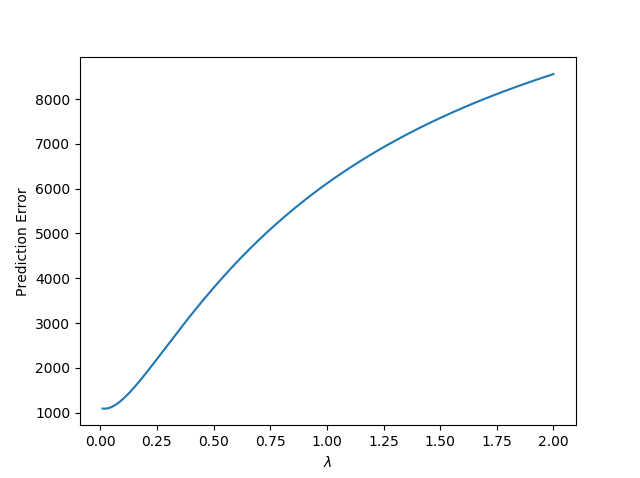
\includegraphics[height=4in]{Figure_1.png}
    \caption{Prediction error as a function of $\lambda$ for question (1.3)}
\end{figure}
\vspace{3cm}

For $\lambda$ = 1, the estimated values of $\beta_{0}$ and $b$ are:
\begin{center}
$\beta_{0} = 
\begin{pmatrix}
-0.1714 \\
-0.3714 \\
0.1460 \\
-0.1330
\end{pmatrix}$

$b = 
\begin{pmatrix}
 0.3226 &  0.7312 & -0.0157 &  0.0241 \\
 0.4002 & -0.0274 &  0.0560 &  0.0945 \\
 0.0332 &  0.0519 &  0.3572 &  0.7226 \\
-0.0685 & -0.0826 &  0.3265 & -0.0234
\end{pmatrix}$
\end{center}
\vspace{5mm}
(1.4) Now, if we want to minimize a slightly modified version of the original function:
\begin{center}
    $F(\beta_{0}, b) = \sum\limits_{k=1}^N|y_{k} - \beta_{0} - b^{T}x_{k}|^{2} + \lambda$ trace($\beta D\beta^{T}$)
\end{center}
where D is now a positive semi-definite $q \times q$ symmetric matrix and $\beta = (\beta_{0}, b^{T})^{T}$. We can define the matrices $\mathcal{X}$ and $\mathcal{Y}$:
\begin{center}
$\mathcal{X} = 
\begin{pmatrix}
\tilde{x}_{1}^{T} \\
\vdots \\
\tilde{x}_{N}^{T}
\end{pmatrix}
,
\mathcal{Y} = 
\begin{pmatrix}
y_{1} \\
\vdots \\
y_{N}
\end{pmatrix}
,$ where 
$\tilde{x} = 
\begin{pmatrix}
1 \\
x(1) \\
\vdots \\
x(d)
\end{pmatrix}$
\end{center}
Take the partial derivative of $F(\beta_{0}, b)$ with respect to $\beta_{0}$, set it equal to 0 and plug in variables:
\begin{center}
    $0 = -2\mathcal{X}^{T}(\mathcal{Y}- \mathcal{X}b) + 2\lambda bD$
    
    $0 = -\mathcal{X}^{T}(\mathcal{Y}- \mathcal{X}b) + \lambda bD$
    
    $0 = \mathcal{X}^{T}\mathcal{X}b + \lambda bD - \mathcal{X}^{T}\mathcal{Y}$
\end{center}
The optimal $\hat{\beta}$ satisfies the "Sylvester Equation":
\begin{center}
    $\mathcal{X}^{T}\mathcal{X}b + \lambda bD = \mathcal{X}^{T}\mathcal{Y}$
\end{center}
\vspace{5mm}
(1.5) The program used to return optimal parameters for $\beta_{0}$ and $b$ for the multivariate problem in question (1.4) is tested using the given dataset for two cases:
\begin{enumerate}
    \item $\lambda$ = 10, $D$ = Id
    \item $\lambda$ = 1000, $D$ is a tridiagonal matrix with -1 above and below the diagonal, and 2 on the diagonal, except $D$(1, 1) = $D(q, q)$ = 1.
\end{enumerate}
The values of $\beta_{0}(j), b(1, j), b(2, j),$ and $b(3, j)$ as functions of $j$ for cases 1 and 2 are shown below in Figures 2 and 3, respectively. While the overall trends for each vector do not change significantly for different values of $\lambda$ and $D$, the amount of noise between the two cases tends to change slightly.
\begin{figure}[h!]
    \centering
    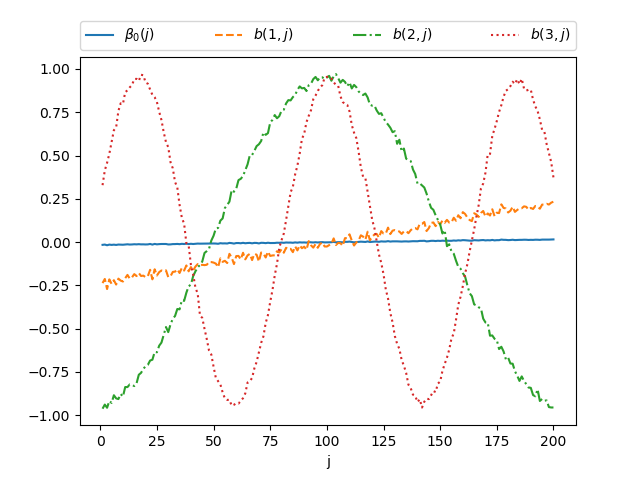
\includegraphics[height=4in]{Figure_2.png}
    \caption{Optimal parameters as a function of $j$ for case 1}
\end{figure}
\begin{figure}[h!]
    \centering
    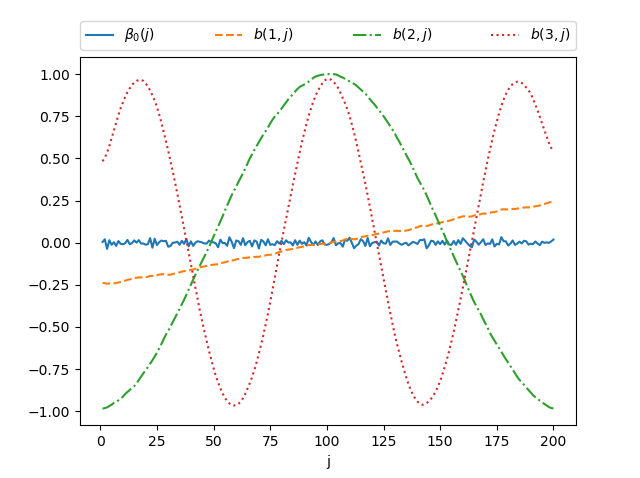
\includegraphics[height=4in]{Figure_3.png}
    \caption{Optimal parameters as a function of $j$ for case 2}
\end{figure}